\subsection{Heurística de Búsqueda Tabú}

 Busqueda Tabu (Tabu search\footnote{Glover, F. "Tabu Search — Part I", ORSA Journal on Computing 1989}) es una estrategia para resolver problemas combinatorios cuya aplicacion es en teoria de grafos y varios problemas de programaciones, entre otros. Este metodo tiene origenes en aplicaciones combinatorias a fines de los 70, y consecuentemente fue aplicado en diversas colecciones de problemas de programacion. El mismo consiste en utilizar el procedimiento de busqueda local\footnote{Ver seccione anterior} para moverse a una mejor solucion en un entorno. Dado que hay veces que no se puede mejorar la solucion la misma permite empeorar parcialmente esta solucion en busca de otras mejores. A su vez esta heuristica concede una estructura llamada $lista\ tabu$ utilizada para varios aspectos, en los que se destacan: guardar movimientos para no repetirlos, guardar caracteristicas o soluciones, por ejemplo. A continuacion mostraremos el pseudocodigo\footnote{Pseudocodigo tomado de la clase de heuristicas correspondiente a Algoritmos y Estructuras III, UBA} que describe al mismo:

\begin{algorithm}[H]
\SetAlgoLined
s$_{0}$ $\leftarrow$ solucion inicial \\
s$^{*}$ $\leftarrow$ s$_{0}$ \\
T $\leftarrow$ lista tabu inicial \\
\While{ no se alcance el criterio de terminacion}{
N $\leftarrow$ vecinos de s no tabu o mejores que s$^{*}$ \\
s $\leftarrow$ mejor solucion en N. \\
\If{ s es mejor que s$^{*}$}
 {s$^{*}$ $\leftarrow$ s} 
Actualizar la lista tabu T }
\end{algorithm}



\subsubsection{Explicación del algoritmo realizado}

 El mismo parte de una solucion provista por el algoritmo de busqueda local, y un valor entero positivo ingresado como parametro llamado $desviacion\_permitida$. A partir de la solucion, el algoritmo va buscando una mejor solucion de la siguiente forma:
\begin{itemize}
 \item Agrega un nodo: Dada una solucion actual (una clique) procede a $agregar$ el mejor nodo\footnote{el que genere mayor frontera a dicha solucion}.
 \item Quita un nodo: Dada una solucion actual procede a $quitar$ el mejor nodo.
\end{itemize}
 De esta manera en cada paso se busca la mejor solucion, en otras palabras, el algoritmo avanza hasta un maximo local. \newline

\begin{figure}[H] %[h] Aqui [b] para button [t] para top
\begin{center}
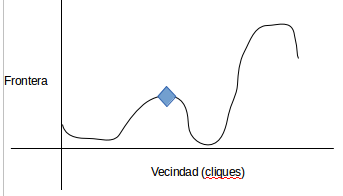
\includegraphics[width=250pt]{../imgs/1_tabu.png}
\caption{Ejemplo}
\end{center}
\end{figure}

 Luego, y a diferencia de la busqueda Local, empezamos a buscar nuevas soluciones pero que no mejoren la solucion. Sin embargo, dentro de las formas que hay de empeorar la solucion, tomamos aquella que empeora lo menos posible. A su vez, a medida que agregamos o quitamos un nodo lo vamos poniendo en la lista tabu. Esto lo hace sin olvidar que siempre que pueda subir lo va a hacer, entonces, si descendiendo se encuentra con que puede volver a ascender, lo va a hacer hasta volver a estar en un maximo local. \newline

\begin{figure}[H] %[h] Aqui [b] para button [t] para top
\begin{center}
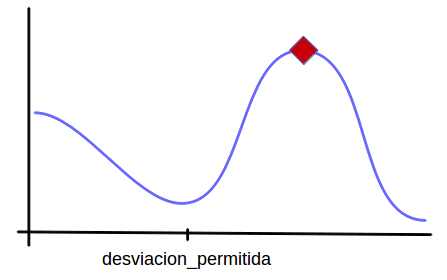
\includegraphics[width=250pt]{../imgs/2_tabu.png}
\caption{Ejemplo}
\end{center}
\end{figure}

Al final el algoritmo retorna la mejor solucion encontrada. \newline

\textbf{Descripcion de la lista tabu} \newline

 A medida que se van agregando o quitando nodos que no mejoran la solucion estos nodos se van marcando como tabu. De esta forma se le asigna una prioridad a cada nodo que depende de cuando fue agregado. A su vez, sea cual sea la prioridad del ultimo agregado, no se puede utilizar en la iteracion siguiente, esto es para evitar ciclar soluciones. Esto lo logramos haciendo que en el peor de los casos solo se puedan usar los nodos tabus que tienen prioridad menor a la mitad de la prioridad maxima. \newline

\textbf{Criterio de terminacion} \newline

 La terminacion de este algoritmo va a estar dada por dos factores, por un lado, la cantidad de iteraciones en que la solucion puede mejorar, y por otro, por la variable $desviacion\_permitida$ ingresada como parametro. El primero es seguro que es acotado ya que el maximo absoluto esta dado por la solucion exacta del problema, entonces, puede haber muchos maximos locales pero ninguno va a superar el maximo absoluto (esto es trivial). Por otro lado, la variable $desviacion\_permitida$ va disminuyendo cada vez que modifico la solucion actual sin mejorarla, es decir, que permitimos avanzar de manera "no creciente" una cantidad $desviacion\_permitida$ de veces. \newline


\begin{algorithm}[H]
    \SetAlgoLined
    \caption{TabuSearch}
    \KwIn{\textbf{Conj(nodos)} $solución\_inicial$, \textbf{Grafo} $g$, \textbf{Entero} $desviacion\_permitida$}
    \KwOut{\textbf{Conj(nodos)} $solución\_final$}

	\textbf{Conj(nodos)} sol$_{0}$,sol$_{1}$ \\ 
	\textbf{Conj(nodos)} $solución\_actual$ $\leftarrow$ LocalSearch($solución\_inicial$, $g$)	\\	
	\textbf{Conj(nodos)} $solución\_final$ $\leftarrow$ $solución\_actual$	\\	
	\textbf{Lista Tabu} $\leftarrow$ $\{\}$\\
	\textbf{Boolean} $Mejore\ la\ frontera$ $\leftarrow$ true

	\While{ $Mejore\ la\ frontera$ $\vee$ 0 $<$ $desviacion\_permitida$}{

	 	sol$_{0}$ $\leftarrow$ Dame Mejor solucion agregando nodo No Tabu ($solución\_inicial$,$solución\_final$) \\
		sol$_{1}$ $\leftarrow$ Dame Mejor solucion quitando nodo No Tabu ($solución\_inicial$,$solución\_final$) \\
		\If{ frontera(sol$_{0}$) $<$ frontera(sol$_{1}$)}
			{sol$_{0}$ $\leftarrow$ sol$_{1}$}
		\eIf{ frontera($solución\_actual$) $<$ frontera(sol$_{1}$)}
			{$solución\_actual$ $\leftarrow$ sol$_{0}$ \\
			$Mejore\ la\ frontera$ $\leftarrow$ true
			}
			{$Mejore\ la\ frontera$ $\leftarrow$ false \\
			 Poner Tabu Nodo utilizado en sol$_{0}$ \\
			 $desviacion\_permitida$ - 1}
		$solución\_actual$ $\leftarrow$ sol$_{0}$ \\
		\If{ frontera($solución\_final$) $<$ frontera($solución\_actual$) } 
		{$solución\_final$ $\leftarrow$ $solución\_actual$}			
	}

    	\textbf{devolver} $solución\_final$ \\

\end{algorithm}

\begin{algorithm}[H]
    \SetAlgoLined
    \caption{Dame Mejor solucion agregando nodo No Tabu}

	$solución\_final$ $\leftarrow$ $solución\_inicial$ sin un nodo cualquiera \\
	\ForAll{$u \in Candidatos\_clique($solución\_inicial$)$}{
	 		\If{$u$ $\notin Nodos(solución\_inicial)$}{
				\eIf{$\neg$ es tabu($u$)}{
		 			\If{frontera($solución\_final$) $<$ frontera( $solución\_inicial$ con $u$) }{
						$solución\_final$ $\leftarrow$ $solución\_inicial$ con $u$}
				}{
					\If{ Es Tabu aceptable ($u$) $\land$ frontera($solución\_final$) $<$ frontera( $solución\_inicial$ con $u$)}
					{$solución\_final$ $\leftarrow$ $solución\_inicial$ con $u$}
				
				}
			}
	}

\end{algorithm}

\begin{algorithm}[H]
    \SetAlgoLined
    \caption{Dame Mejor solucion quitando nodo No Tabu}

	$solución\_final$ $\leftarrow$ $solución\_inicial$ sin un nodo cualquiera \\
	\ForAll{$u \in$ Nodos($solución$\_$inicial$)}{
		\eIf{$\neg$ es tabu($u$)}{
	 		\If{frontera($solución\_final$) $<$ frontera( $solución\_inicial$ sin $u$)}{
	 			$solución\_final$ $\leftarrow$ $solución\_inicial$ sin $u$}
		}{
				\If{Es Tabu aceptable ($u$) $\land$ frontera($solución\_final$) $<$ frontera($solución\_inicial$ con $u$)}
					{$solución\_final$ $\leftarrow$ $solución\_inicial$ con $u$}
		}
	}

\end{algorithm}

Donde:
\begin{itemize}
 \item $desviacion$\_$permitida$ Dice la cantidad de veces que se agrega o quita un nodo por iteracion (empeorando la solución parcial).
 \item frontera : Dice, dada una solución como parametro, el numero de nodos adyacentes a la frontera (es lo que pide maximizar el enunciado).
 \item Candidatos$\_$clique : Dice los nodos que pertenecen a la clique maxima de los nodos pasados como parametro.
 \item Nodos : Da los nodos pertenecientes a la solución pasada como parametro.
 \item Es Tabu aceptable : Un nodo perteneciente a la lista tabu es aceptable si su prioridad es menor a la mitad de la prioridad maxima.
\end{itemize}

\subsubsection{Complejidad Temporal}
\subsubsection{Instancias problemáticas}
\subsubsection{Experimentación}
